%% Week 44 -- Convolutional neural networks from the start, following the
%% 2025 week-45 lecture notes (doc/pub/week45/ipynb/week45.ipynb): what a CNN
%% is and why, the mathematics of convolution with its examples (polynomial
%% multiplication, Toeplitz matrices, padding, cross-correlation, the 3x3 /
%% 2x2 example, the flattened matrix, output sizes and parameter counts),
%% filters at work (a digit, a drawn house, houses in a photograph), pooling,
%% and complete PyTorch and TensorFlow/Keras programs on MNIST compared with
%% the dense network of Project 2.  One idea per frame.
%% Figures: figslides/ of the 2025 week-45 folder (nn.jpeg, cnn.jpeg,
%% deepcnn.png, discreteconv1.png, maxpooling.png), week43_convolution.pdf,
%% and week44_*.pdf from make_week44_figures.py (Parts 1-4 and 6).  The
%% companion notebook week44.ipynb carries all the code, the from-scratch
%% implementation and the gradient checks (not on the slides).
%% Book references (book.aux 2026-10-25, after the chapter-10 revision that
%% added Sections 10.2 (vocabulary), 10.7 (filters at work), 10.12.6 (dense
%% vs CNN on MNIST) and 10.13 (Fourier filters)): Chapter 10, Sections
%% 10.1-10.7 and 10.10-10.13; Eqs 10.3-10.4 (convolution), 10.5-10.8
%% (polynomials, Toeplitz), 10.12-10.13 (padding, cross-correlation),
%% 10.14-10.16 (2D, the layer), 10.17-10.18 (sizes, parameters), 10.19
%% (unrolled), 10.21 (pooling), 10.26-10.28 (the house filters, NCC),
%% 10.29-10.33 (backprop), 10.34 (im2col), 10.35 (arch); Table 10.1, Table
%% 10.2, Table 10.3 (dense vs CNN); the Fourier material is Section 10.13.
%% Build:  pdflatex week44slides.tex  (twice)
\documentclass[10pt,aspectratio=169]{beamer}
\usetheme{red_plain}
\usepackage[T1]{fontenc}
\usepackage[utf8]{inputenc}
\usepackage{amsmath,amssymb,bm}
\usepackage{graphicx}
\usepackage{listings}
\usepackage{xcolor}
\usepackage{booktabs}
\graphicspath{{../BookFigures/chapter10_convolutional_networks/}{../../pub/week45/ipynb/figslides/}{./}}

%% ---- code listings
\definecolor{codebg}{rgb}{0.97,0.97,0.97}
\lstset{language=Python,basicstyle=\ttfamily\scriptsize,backgroundcolor=\color{codebg},
  keywordstyle=\color{blue!70!black}\bfseries,commentstyle=\color{green!45!black},
  stringstyle=\color{red!60!black},showstringspaces=false,frame=single,
  framerule=0pt,xleftmargin=4pt,xrightmargin=4pt,breaklines=true,columns=fullflexible}

%% ---- the "pause and think" question frames
\newcounter{insight}
\newenvironment{insight}[1][]{%
  \stepcounter{insight}%
  \begin{frame}{Pause and think \arabic{insight}: #1}%
  \setbeamercolor{block title}{bg=structure.fg,fg=white}%
  \setbeamercolor{block body}{bg=structure.fg!8}%
  \small
}{\end{frame}}
\newcommand{\question}[1]{\begin{block}{Question}#1\end{block}}
\newcommand{\answer}[1]{\pause\begin{block}{Answer}#1\end{block}}

\setbeamertemplate{footline}[frame number]
\setbeamerfont{block title}{size=\small}
\setbeamertemplate{blocks}[rounded][shadow=false]
\setbeamercovered{invisible}

\title{Week 44: Convolutional Neural Networks}
\subtitle{What they are and why, the mathematics of convolution, filters at
  work, pooling, and complete PyTorch and TensorFlow programs on MNIST\\[3pt]
  \small With pauses for questions}
\author{Morten Hjorth-Jensen}
\institute{Department of Physics and Center for Computing in Science Education,\\
  University of Oslo, Norway}
\date{}

\begin{document}

\begin{frame}
\titlepage
\end{frame}

\begin{frame}{Plan for week 44}
\small
\textbf{Monday lecture (2$\times$45 min):}
\begin{enumerate}
  \item \textbf{What a convolutional network is, and why} (15 min): the
        same neurons, weights and biases as before -- plus one assumption,
        that the input is an image.
  \item \textbf{The mathematics of convolution} (35 min): the definition,
        polynomial multiplication as the first example, Toeplitz matrices,
        padding and stride, cross-correlation (what the libraries compute),
        two dimensions, a $3\times3$ example by hand, output sizes and
        parameter counts.
  \item \textbf{Filters at work} (15 min): edge filters on a digit, on a
        drawn house and on a photograph of houses; a filter that finds
        windows; what a trained network learns; pooling.
  \item \textbf{CNNs in code} (20 min): the same network in TensorFlow/Keras
        and in PyTorch on MNIST, compared with the dense network of Project 2.
  \item \textbf{Fourier filters} (10 min): the convolution theorem, filtering
        by multiplication, the photograph in Fourier space, a CNN layer in
        Fourier language, and where Fourier filters are used.
\end{enumerate}
\textbf{Tuesday (flipped classroom):} cross-validation for your Project 2
network -- the week-44 exercises (deadline \textbf{Friday October 30}).
Project 2 is due November 6.\\[3pt]
\textbf{Reading:} Chapter 10 of the lecture notes, Sections 10.1--10.7 and
10.10--10.13 (10.7: filters at work; 10.13: Fourier filters); Goodfellow et
al.\ Chapter 9; Raschka et al.\ Chapters 14--15.
The code of today is in \texttt{week44.ipynb}.
\end{frame}

%% =====================================================================
\section{What a CNN is, and why}
\begin{frame}{Convolutional neural networks: recognising images}
\small
Convolutional neural networks (CNNs) were developed in the 1990s for
character recognition.  Today they are a central element of the success of
deep learning, above all for images.

\medskip
\textbf{CNNs are very similar to the neural networks we have seen.}
\begin{itemize}
  \item They are made up of neurons with learnable weights and biases.
  \item Each neuron receives some inputs, performs a dot product and
        (optionally) applies a non-linearity.
  \item The whole network is a single differentiable function, from raw
        pixels to class scores.
  \item There is a loss function on the last (fully connected) layer --
        the softmax cross entropy for classification -- and everything we
        know about training applies: backpropagation, gradient descent, Adam.
\end{itemize}

\medskip
\begin{block}{So what is the difference?}
CNN architectures make the \emph{explicit assumption that the inputs are
images}.  This lets us build certain properties into the architecture,
which makes the forward pass more efficient and reduces the number of
parameters enormously.
\end{block}
\end{frame}

\begin{frame}{Neural networks are affine transformations -- images have structure}
\small
\begin{columns}[T]
\begin{column}{0.5\textwidth}
\begin{block}{A dense layer}
A vector comes in, is multiplied by a weight matrix, a bias is added, and
an activation function is applied:
\[
  \bm{a}=f(\bm{W}\bm{x}+\bm{b}).
\]
This works for \emph{any} input -- an image, a sound clip, a table --
because whatever its shape, the input can be flattened into a vector
first.
\end{block}
\end{column}
\begin{column}{0.48\textwidth}
\begin{block}{What flattening throws away}
Images, sound clips and many similar data share three properties:
\begin{itemize}
  \item they are stored as multi-dimensional arrays (the pixels);
  \item one or more axes have an \emph{ordering} that matters (width and
        height of an image, time in a sound clip);
  \item one axis, the \emph{channel} axis, holds different views of the
        same data (red, green and blue; left and right audio channel).
\end{itemize}
\end{block}
\end{column}
\end{columns}
\medskip
An affine transformation treats all axes the same way: the topology is not
used.  A \textbf{discrete convolution} is a linear transformation that
\emph{keeps} the ordering.  It is \emph{sparse} (only a few input units
contribute to a given output unit) and it \emph{reuses parameters} (the
same weights are applied at many places in the input).
\end{frame}

\begin{frame}{Regular neural networks do not scale to full images}
\small
\begin{columns}[T]
\begin{column}{0.5\textwidth}
\begin{itemize}
  \item A colour image of $32\times32$ pixels has $32\times32\times3=3072$
        numbers: every neuron of the first hidden layer needs $3072$
        weights.  Still manageable.
  \item A $200\times200$ colour image: $120\,000$ weights \emph{per
        neuron}.  With a few hundred neurons we are at tens of millions of
        parameters -- wasteful, and an invitation to overfit.
\end{itemize}
\begin{block}{A sound example}
An input of length $d=10^{6}$ and one hidden layer of $10^{4}$ nodes: the
weight matrix has $10^{4}\times10^{6}=10^{10}$ entries.  With the $10^{4}$
biases and the output layer,
\[
  \mathrm{NumberParameters}=10^{10}+10^{4}+10^{4}+1\approx10^{10},
\]
ten billion parameters -- to decide whether the clip is a human voice.
\end{block}
\end{column}
\begin{column}{0.48\textwidth}
\begin{center}
\includegraphics[width=0.95\textwidth]{nn}\\
\scriptsize A regular three-layer neural network: every input connected to
every hidden neuron.
\end{center}
\end{column}
\end{columns}
\end{frame}

\begin{frame}{The CNN answer: neurons arranged in three dimensions}
\small
\begin{columns}[T]
\begin{column}{0.5\textwidth}
\begin{itemize}
  \item The layers of a CNN have neurons arranged in \emph{width, height
        and depth} -- a volume.  (``Depth'' here is the third dimension of
        one layer, not the number of layers.)
  \item The input volume of a $32\times32$ colour image is
        $32\times32\times3$.
  \item A neuron is connected only to a \emph{small region} of the layer
        before it -- not to all of it.
  \item At the end the volume is reduced to a single vector of class
        scores, $1\times1\times10$ for ten classes.
\end{itemize}
\end{column}
\begin{column}{0.48\textwidth}
\begin{center}
\includegraphics[width=0.9\textwidth]{cnn}\\
\scriptsize Every layer transforms a 3D input volume into a 3D output
volume.  The red input layer holds the image: width and height are the
image size, the depth is 3 (R, G, B).
\end{center}
\end{column}
\end{columns}
\begin{block}{Two principles behind the construction}
\textbf{Locality:} neighbouring pixels are related, far-away ones much
less.  \textbf{Repetition:} the same pattern -- an edge, a corner --
appears at many places.  So: connect a neuron to a small neighbourhood
only, and use the \emph{same} weights at every place.  That operation is
a \emph{convolution}, a \emph{filtering}.
\end{block}
\end{frame}

\begin{frame}{Filters: hand-made in signal processing, learned in a CNN}
\small
In signal and image processing one \emph{designs} filters: a filter is a
small array of weights, and ``applying the filter'' is a convolution of the
image with it.  There are filters for smoothing, for edge detection, for
reshaping frequencies -- hand-crafted, from experience.

\medskip
\begin{block}{The idea of a convolutional network}
Do not design the filters: \emph{learn} them from the data, use many of
them at once, and put non-linear activation functions between layers of
filters so that simple patterns found by the first layer (edges) can be
combined into more complex ones (corners, windows, roofs, houses) by the
next.
\end{block}

\medskip
Today we first make the word ``convolution'' precise (Part 2), then look at
what hand-made filters do to a digit and to a house (Part 3), and finally
let the libraries learn the filters (Part 4).
\end{frame}

\begin{frame}{The layers used to build a CNN}
\small
A simple CNN is a sequence of layers, and every layer transforms one volume
of activations into another through a differentiable function.  Three kinds
of layer, stacked:
\begin{itemize}
  \item \textbf{INPUT} $[32\times32\times3]$: the raw pixel values, width
        32, height 32, three colour channels.
  \item \textbf{CONV}: each neuron computes a dot product between its
        weights and a small region of the input it is connected to.  With
        12 filters the output is $[32\times32\times12]$.
  \item \textbf{RELU}: the elementwise $\max(0,x)$; the size is unchanged,
        $[32\times32\times12]$.
  \item \textbf{POOL}: downsampling along width and height, for example to
        $[16\times16\times12]$.
  \item \textbf{FC} (fully connected): computes the class scores,
        $[1\times1\times10]$; every neuron sees all the numbers of the
        previous volume, as in an ordinary network.
\end{itemize}
\begin{block}{Which layers have parameters}
CONV and FC have weights and biases, trained by gradient descent so that
the class scores agree with the labels.  RELU and POOL are fixed functions
with no parameters.  CONV, FC and POOL have \emph{hyperparameters} (filter
size, number of filters, stride, \dots); RELU has none.
\end{block}
\end{frame}

\begin{frame}{A deep CNN model (from Raschka et al.)}
\begin{center}
\includegraphics[width=0.92\textwidth]{deepcnn}
\end{center}
\small
Convolution -- pooling -- convolution -- pooling -- flatten -- fully
connected -- fully connected.  The volumes shrink in width and height and
grow in depth: $28\times28\times1\to28\times28\times32\to14\times14\times32
\to14\times14\times64\to7\times7\times64\to1024\to10$.  This is the
network we will run in PyTorch and Keras in Part 4, with $3\times3$ filters
instead of $5\times5$.
\end{frame}

%% =====================================================================
\section{The mathematics of convolution}
\begin{frame}{The mathematics of CNNs: convolution}
\small
Convolution is an operation on two functions that produces a third: it
expresses how the shape of one is modified by the other.  It appears in
statistics, signal processing, differential equations, linear algebra --
and machine learning.
\begin{block}{Definition, one dimension}
For a continuous input $x(a)$ and a \emph{weight function} or
\emph{kernel} $w$,
\[
  y(t)=\int x(a)\,w(t-a)\,da ,\qquad\text{written } y=x*w .
\]
The discrete version, for sequences, is
\[
  y(t)=\sum_{a=-\infty}^{\infty}x(a)\,w(t-a).
\]
\end{block}
\begin{itemize}
  \item The operation is \emph{commutative}: $x*w=w*x$ (substitute
        $a\to t-a$ in the sum).
  \item It is \emph{linear} in each argument.
  \item Undoing a convolution is called deconvolution.
\end{itemize}
What does it mean, and how can we use it?  Let us look at a familiar
example first.
\end{frame}

\begin{frame}{Example 1: polynomial multiplication}
\small
Multiply a polynomial of degree two by one of degree three,
\[
  p(t)=\alpha_0+\alpha_1t+\alpha_2t^{2},\qquad
  s(t)=\beta_0+\beta_1t+\beta_2t^{2}+\beta_3t^{3}.
\]
The product is a polynomial of degree five,
$z(t)=\delta_0+\delta_1t+\dots+\delta_5t^{5}$, with coefficients
\begin{align*}
  \delta_0&=\alpha_0\beta_0\\
  \delta_1&=\alpha_1\beta_0+\alpha_0\beta_1\\
  \delta_2&=\alpha_0\beta_2+\alpha_1\beta_1+\alpha_2\beta_0\\
  \delta_3&=\alpha_1\beta_2+\alpha_2\beta_1+\alpha_0\beta_3\\
  \delta_4&=\alpha_2\beta_2+\alpha_1\beta_3\\
  \delta_5&=\alpha_2\beta_3 .
\end{align*}
Look at the indices: in every product the two indices \emph{add up to the
index on the left}.
\end{frame}

\begin{frame}{Example 1 continued: the product is a discrete convolution}
\small
Set $\alpha_i=0$ outside $i\in\{0,1,2\}$ and $\beta_j=0$ outside
$j\in\{0,1,2,3\}$.  Then every line of the previous frame is one instance
of
\[
  \delta_j=\sum_{i=-\infty}^{\infty}\alpha_i\,\beta_{j-i}=(\alpha*\beta)_j ,
\]
a discrete convolution of the two coefficient sequences.  Since only three
$\alpha$'s are non-zero,
\[
  \delta_i=\sum_{k=0}^{m-1}\alpha_k\,\beta_{i-k},\qquad m=3 ,
\]
where $m$ is the length of $\bm{\alpha}$ and $n=4$ is the length of
$\bm{\beta}$.
\begin{block}{Polynomial multiplication \emph{is} convolution}
Not an analogy: multiplying two polynomials convolves their coefficient
sequences.  The length of the result is $m+n-1=6$.
\end{block}
\end{frame}

\begin{frame}{Example 1 continued: a matrix--vector product}
\small
Only finitely many coefficients are non-zero, so the convolution can be
written as a matrix times a vector,
\[
  \bm{\delta}=
  \begin{bmatrix}\alpha_0&0&0&0\\ \alpha_1&\alpha_0&0&0\\
  \alpha_2&\alpha_1&\alpha_0&0\\ 0&\alpha_2&\alpha_1&\alpha_0\\
  0&0&\alpha_2&\alpha_1\\ 0&0&0&\alpha_2\end{bmatrix}
  \begin{bmatrix}\beta_0\\ \beta_1\\ \beta_2\\ \beta_3\end{bmatrix}
  \quad\text{or, equally,}\quad
  \bm{\delta}=
  \begin{bmatrix}\beta_0&0&0\\ \beta_1&\beta_0&0\\ \beta_2&\beta_1&\beta_0\\
  \beta_3&\beta_2&\beta_1\\ 0&\beta_3&\beta_2\\ 0&0&\beta_3\end{bmatrix}
  \begin{bmatrix}\alpha_0\\ \alpha_1\\ \alpha_2\end{bmatrix},
\]
the second form because convolution is commutative.
\begin{block}{Toeplitz matrices}
A matrix whose descending diagonals are constant, $a_{ij}=a_{i-j}$, is a
\emph{Toeplitz} matrix.  Both matrices above are Toeplitz (and not
square).  Every linear convolution is a Toeplitz matrix times a vector --
and the other way round.  Toeplitz matrices are closely connected with
Fourier series: convolution becomes multiplication in Fourier space.
\end{block}
\scriptsize
The matrices are for \emph{reasoning}.  In code we never allocate them; we
compute the sum with the few non-zero terms it has.
\end{frame}

\begin{insight}[the polynomial product by hand and by \texttt{numpy}]
\question{Take $\bm{\alpha}=(1,2,3)$, so $p(t)=1+2t+3t^{2}$, and
$\bm{\beta}=(4,-1,0.5,2)$.  Compute $\bm{\delta}=\bm{\alpha}*\bm{\beta}$
from the six lines two frames back.  Then check it with three lines of
Python.}
\answer{$\delta_0=4$, $\delta_1=2\cdot4+1\cdot(-1)=7$,
$\delta_2=1\cdot0.5+2\cdot(-1)+3\cdot4=10.5$,
$\delta_3=2\cdot0.5+3\cdot(-1)+1\cdot2=0$,
$\delta_4=3\cdot0.5+2\cdot2=5.5$, $\delta_5=3\cdot2=6$:
$z(t)=4+7t+10.5t^{2}+5.5t^{4}+6t^{5}$.\\[3pt]
\texttt{alpha, beta = np.array([1., 2., 3.]), np.array([4., -1., 0.5, 2.])}\\
\texttt{np.polynomial.polynomial.polymul(alpha, beta)}\quad\emph{gives} [4.\ 7.\ 10.5\ 0.\ 5.5\ 6.]\\
\texttt{np.convolve(alpha, beta)}\quad\emph{gives the same six numbers.}\\[3pt]
\texttt{np.convolve} does not know about polynomials; it computes
$\sum_k\alpha_k\beta_{i-k}$.  The notebook also builds the $6\times4$
Toeplitz matrix and multiplies: the same six numbers a third time.}
\end{insight}

\begin{frame}{Generalising: a filter $\bm{w}$ and an input $\bm{x}$}
\small
Rename $\bm{\alpha}$ (length $m=3$) as the \textbf{filter} or
\textbf{weights} $\bm{w}$, and $\bm{\beta}$ (length $n=4$) as the
\textbf{input} $\bm{x}$; the result $\bm{\delta}$ becomes the
\textbf{output} $\bm{y}$.  We always assume $m\le n$: the filter is
small, the input is large.
\[
  y(i)=(x*w)(i)=\sum_{k=0}^{m-1}w(k)\,x(i-k).
\]
\begin{block}{A problem with the indices}
$\bm{x}$ has the components $x(0),x(1),x(2),x(3)$, and $\bm{y}$ has six,
$i=0,\dots,5$.  The sum then asks for $x(-1)$, $x(-2)$ (for $i=0$) and
$x(4)$, $x(5)$ (for $i=5$), which do not exist.  For the polynomials they
were simply zero.  In general we have to \emph{decide} what they are.
\end{block}
\end{frame}

\begin{frame}{Padding}
\small
The solution is \textbf{padding}: add $P$ zeros before $x(0)$ and $P$ zeros
after $x(3)$.  With $P=2$ the input grows from $n=4$ to $n+2P=8$:
\[
  x(0)=0,\ x(1)=0,\ x(2)=\beta_0,\ x(3)=\beta_1,\ x(4)=\beta_2,\ x(5)=\beta_3,\
  x(6)=0,\ x(7)=0 .
\]
Now every index exists, and for $i=0,\dots,5$
\[
  y(i)=\sum_{k=0}^{m-1}w(k)\,x\bigl(i+(m-1)-k\bigr).
\]
\begin{block}{Check against the polynomial product}
\begin{align*}
  y(0)&=x(2)w(0)+x(1)w(1)+x(0)w(2)=\beta_0\alpha_0+0+0=\delta_0,\\
  y(4)&=x(6)w(0)+x(5)w(1)+x(4)w(2)=0+\beta_3\alpha_1+\beta_2\alpha_2=\delta_4,\\
  y(5)&=x(7)w(0)+x(6)w(1)+x(5)w(2)=0+0+\beta_3\alpha_2=\delta_5 .
\end{align*}
\end{block}
The padding $P$ is a \emph{hyperparameter} of the architecture, like the
number of hidden nodes.  A second one, the \emph{stride} $S$, comes in a
moment.
\end{frame}

\begin{frame}{Flip the filter, and the sum is a dot product -- cross-correlation}
\small
Look at $y(0)=x(2)w(0)+x(1)w(1)+x(0)w(2)$: the input runs \emph{forwards},
the filter \emph{backwards}.  Define the flipped filter
$\tilde w(0)=w(2)$, $\tilde w(1)=w(1)$, $\tilde w(2)=w(0)$.  Then
\[
  y(0)=x(0)\tilde w(0)+x(1)\tilde w(1)+x(2)\tilde w(2),
\]
a plain \textbf{dot product} of the filter with the \emph{patch}
$x(0{:}3)$ of the input, and $y(i)$ is the dot product with the patch
$x(i{:}i+m)$: slide the filter along the input, take a dot product at
every position.
\begin{block}{Cross-correlation: what the libraries compute}
Nobody flips the filter in practice.  Instead of the convolution
$y(i)=\sum_kw(k)\,x(i-k)$ one computes
\[
  y(i)=\sum_{k}w(k)\,x(i+k),
\]
the \textbf{cross-correlation}.  TensorFlow, PyTorch and our own code all
implement this, and all of them \emph{call} it convolution.  The two differ
only by the order of the filter weights, and since the weights are
\emph{learned}, it makes no difference.  Padding and stride work the same
way for both.
\end{block}
\end{frame}

\begin{frame}{Two dimensions}
\small
An image is a two-dimensional array $X$, and a filter is a small
two-dimensional array $W$ (the \emph{kernel}).  The convolution is
\[
  Y(i,j)=(X*W)(i,j)=\sum_m\sum_nX(m,n)\,W(i-m,j-n),
\]
or, by commutativity, with the filter indices running over the small
range,
\[
  Y(i,j)=\sum_m\sum_nX(i-m,j-n)\,W(m,n),
\]
which is the form one implements.  And as in one dimension, the libraries
compute the \textbf{cross-correlation}
\[
  \boxed{\;Y(i,j)=\sum_m\sum_nX(i+m,\,j+n)\,W(m,n)\;}
\]
and call it convolution.  Read it as: put the filter with its corner at
$(i,j)$, multiply the overlapping numbers pairwise, add them up, write
the sum into $Y(i,j)$.  Then move the filter.
\end{frame}

\begin{frame}{A simple example: a $3\times3$ input and a $2\times2$ filter}
\small
\[
  \bm{X}=\begin{bmatrix}x_{00}&x_{01}&x_{02}\\ x_{10}&x_{11}&x_{12}\\
  x_{20}&x_{21}&x_{22}\end{bmatrix},\qquad
  \bm{W}=\begin{bmatrix}w_{00}&w_{01}\\ w_{10}&w_{11}\end{bmatrix}.
\]
The \textbf{stride} $S$ says how far the filter moves between two
positions.  With $S=1$ it starts at $x_{00}$ and visits every $2\times2$
submatrix, column by column, row by row:
\[
  \bm{Y}=\begin{bmatrix}
  x_{00}w_{00}+x_{01}w_{01}+x_{10}w_{10}+x_{11}w_{11} &
  x_{01}w_{00}+x_{02}w_{01}+x_{11}w_{10}+x_{12}w_{11}\\[2pt]
  x_{10}w_{00}+x_{11}w_{01}+x_{20}w_{10}+x_{21}w_{11} &
  x_{11}w_{00}+x_{12}w_{01}+x_{21}w_{10}+x_{22}w_{11}
  \end{bmatrix}.
\]
\begin{block}{With numbers}
$\bm{X}=\bigl(\begin{smallmatrix}1&2&3\\4&5&6\\7&8&9\end{smallmatrix}\bigr)$,
$\bm{W}=\bigl(\begin{smallmatrix}1&2\\3&4\end{smallmatrix}\bigr)$:
$Y_{00}=1\cdot1+2\cdot2+4\cdot3+5\cdot4=37$, and
$\bm{Y}=\bigl(\begin{smallmatrix}37&47\\67&77\end{smallmatrix}\bigr)$.
A $3\times3$ input and a $2\times2$ filter give a $2\times2$ output.
\end{block}
\scriptsize
For pictures of every case (padding, stride, dilation) see the repository
\emph{Arithmetic of deep learning} by Dumoulin and Visin,
\texttt{github.com/vdumoulin/conv\_arithmetic}.
\end{frame}

\begin{frame}{The same example as a matrix--vector product}
\small
Flatten the input into a vector $\bm{X}'$ of length $9$ and write the
filter as a $4\times9$ matrix $\bm{W}'$:
\[
  \bm{X}'=\begin{bmatrix}x_{00}\\x_{01}\\x_{02}\\x_{10}\\x_{11}\\x_{12}\\x_{20}\\x_{21}\\x_{22}\end{bmatrix},
  \qquad
  \bm{W}'=\begin{bmatrix}
  w_{00}&w_{01}&0&w_{10}&w_{11}&0&0&0&0\\
  0&w_{00}&w_{01}&0&w_{10}&w_{11}&0&0&0\\
  0&0&0&w_{00}&w_{01}&0&w_{10}&w_{11}&0\\
  0&0&0&0&w_{00}&w_{01}&0&w_{10}&w_{11}
  \end{bmatrix}.
\]
Then $\bm{W}'\bm{X}'$ is a vector of length $4$ holding exactly the four
entries of $\bm{Y}$: the convolution with stride $1$ \emph{is} this
matrix--vector product (with the numbers of the previous frame:
$(37,47,67,77)$).
\begin{block}{What the matrix shows}
A convolutional layer is a dense layer whose weight matrix has a very
special form: most entries are zero (\emph{locality}), and the non-zero
entries are the same four numbers repeated (\emph{parameter sharing}).
A dense $4\times9$ layer would have $36$ free parameters; this one has $4$.
\end{block}
\end{frame}

\begin{frame}{The convolution stage: hyperparameters, output size, parameters}
\small
The input is a \emph{volume} of width $W_1$, height $H_1$ and depth $D_1$
($D_1=3$ for colour, $1$ for grey).  The convolution stage adds, besides the
weights and biases of the filters, four hyperparameters:
\begin{itemize}
  \item $K$, the number of filters (common values $32,64,128,\dots$);
  \item $F$, the filter's spatial extent ($F\times F$);
  \item $S$, the stride;
  \item $P$, the padding.
\end{itemize}
\begin{columns}[T]
\begin{column}{0.5\textwidth}
\begin{block}{The output volume}
\[
  W_2=\frac{W_1-F+2P}{S}+1,\qquad H_2=\frac{H_1-F+2P}{S}+1,\qquad D_2=K .
\]
\end{block}
\begin{block}{Parameters to train}
Each filter has $F\times F\times D_1$ weights and one bias:
\[
  (F\times F\times D_1)\times K+K\ \text{biases}.
\]
\end{block}
\end{column}
\begin{column}{0.46\textwidth}
\begin{block}{Common settings}
\begin{tabular}{@{}lll@{}}
$F=3$ & $S=1$ & $P=1$ \quad(size unchanged)\\
$F=5$ & $S=1$ & $P=2$ \quad(size unchanged)\\
$F=5$ & $S=2$ & $P$ open \quad(size halved)\\
$F=1$ & $S=1$ & $P=0$ \quad(mixes channels only)
\end{tabular}
\end{block}
\scriptsize A stride is a form of \emph{subsampling}: moving the filter
in hops of two is the same as moving it in hops of one and keeping every
second output.
\end{column}
\end{columns}
\end{frame}

\begin{frame}{Example of a CNN setup}
\small
An input volume of $32\times32\times3$ (three colour channels).  We apply
a $5\times5$ filter ten times ($K=10$) with stride $S=1$ and padding $P=0$.
\begin{itemize}
  \item Output size: $(32-5)/1+1=28$, so ten feature maps of $28\times28$ --
        the output volume is $28\times28\times10$.
  \item Parameters per filter: $5\times5\times3+1=76$ (the last one is the
        bias); for ten filters, $760$ parameters.
  \item A dense layer producing the same $7840$ outputs from the $3072$
        inputs would have $3072\times7840\approx2.4\times10^{7}$ weights.
\end{itemize}
\begin{center}
\includegraphics[width=0.5\textwidth]{discreteconv1}\\
\scriptsize The general discrete convolution (Raschka et al.): a
$3\times3$ kernel on an $8\times8$ input padded with one ring of zeros
($P=1$) gives an $8\times8$ output.
\end{center}
\end{frame}

\begin{insight}[count the parameters]
\question{Same $32\times32\times3$ input.  How many parameters does a
layer of $32$ filters of size $3\times3$ have ($S=1$, $P=0$), and what is
the output volume?  And for MNIST, $28\times28\times1$, with $32$ filters
of size $3\times3$, $S=1$, $P=1$?}
\answer{$3\times3\times3+1=28$ parameters per filter, $28\times32=896$ in
total; output $(32-3)/1+1=30$, so $30\times30\times32$.  For MNIST:
$3\times3\times1+1=10$ per filter, $320$ in total; with $P=1$ the size is
unchanged, $(28-3+2)/1+1=28$, output $28\times28\times32$.  Note what does
\emph{not} enter the parameter count: the image size.  The same $320$
numbers serve a $28\times28$ image and a $4096\times4096$ one -- that is
parameter sharing.  A dense layer from $784$ inputs to $100$ hidden nodes,
the network of week 41, has $78\,500$.}
\end{insight}

%% =====================================================================
\section{Filters at work}
\begin{frame}{Filters at work, 1: three hand-made filters on a digit}
\begin{center}
\includegraphics[width=0.82\textwidth]{week43_convolution}
\end{center}
\small
MNIST test image 8 (a five) and three $3\times3$ filters, no padding, so
$28\to26$.  \textbf{Vertical edges:} the Sobel filter
$\bigl(\begin{smallmatrix}-1&0&1\\-2&0&2\\-1&0&1\end{smallmatrix}\bigr)$
is a derivative along a row: positive (red) where the ink starts, negative
(blue) where it ends, zero inside a stroke.  \textbf{Horizontal edges:} its
transpose, a derivative down a column.  \textbf{Blur:} the $\tfrac19$ mean of
a $3\times3$ patch, a low-pass filter.  Each output is one \emph{feature
map}.  With $K=3$ filters a layer makes all three at once, with
$3\times(9+1)=30$ parameters.
\end{frame}

\begin{frame}{Filters at work, 2: a house (\texttt{week44\_house.pdf})}
\begin{center}
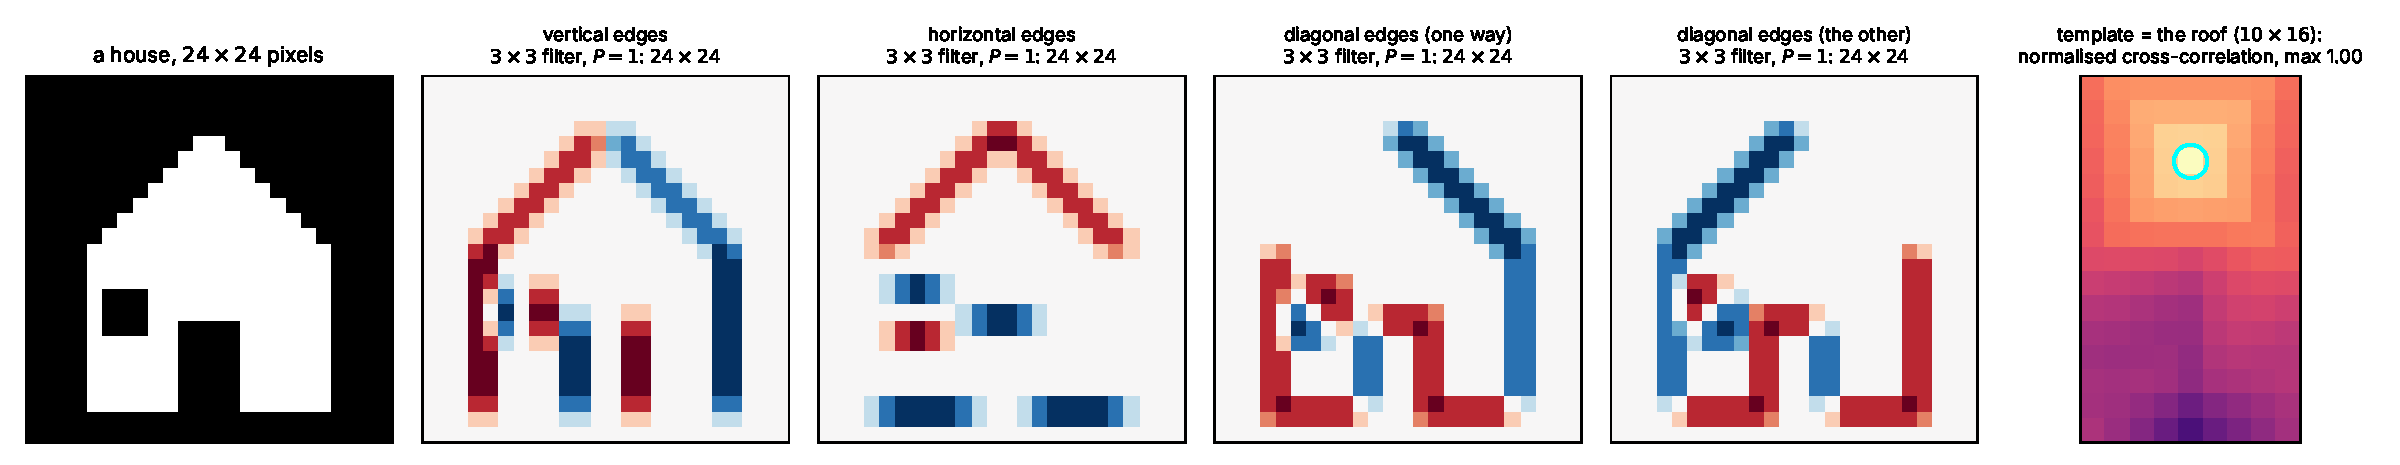
\includegraphics[width=0.99\textwidth]{week44_house}
\end{center}
\small
A $24\times24$ drawing: walls, a gabled roof, a door and a window.  Four
$3\times3$ filters with $P=1$ (the maps keep the size): the vertical-edge
filter finds the walls and the sides of door and window, the horizontal
one the floor, the lintels and the roof as a whole, and the two diagonal
filters each pick out \emph{one} slope of the roof.  The last panel uses
the roof itself, cut out of the picture, as a $10\times16$ filter: the
normalised cross-correlation is $1.00$ exactly where the roof is and
smaller everywhere else -- a filter that \emph{detects a roof}.
\end{frame}

\begin{frame}{The filters of the house, written out}
\scriptsize
\begin{columns}[T]
\begin{column}{0.5\textwidth}
Every map is the cross-correlation
$Y(i,j)=\sum_{m,n}X(i+m-1,\,j+n-1)\,W(m,n)$ with $P=1$ (one ring of
zeros), so $24\times24\to24\times24$.
\begin{block}{The four $3\times3$ edge filters}
\[
  W_{\mathrm{vert}}=\begin{pmatrix}-1&0&1\\-2&0&2\\-1&0&1\end{pmatrix},\qquad
  W_{\mathrm{hor}}=\begin{pmatrix}-1&-2&-1\\0&0&0\\1&2&1\end{pmatrix},
\]
\[
  W_{\diagup}=\begin{pmatrix}0&1&2\\-1&0&1\\-2&-1&0\end{pmatrix},\qquad
  W_{\diagdown}=\begin{pmatrix}2&1&0\\1&0&-1\\0&-1&-2\end{pmatrix}.
\]
\end{block}
$W_{\mathrm{vert}}$ is the Sobel operator: the central difference along
the row, $X(i,j+1)-X(i,j-1)$, averaged over three rows with weights
$(1,2,1)$ -- a smoothed $\partial X/\partial x$.
$W_{\mathrm{hor}}=W_{\mathrm{vert}}^{T}$ is $\partial X/\partial y$.  The
diagonal pair are the same differences along the two diagonals (Sobel
rotated by $45^{\circ}$).  All four have weights summing to zero: a
constant region gives $0$; only \emph{changes} of intensity respond.
\end{column}
\begin{column}{0.48\textwidth}
\begin{block}{The roof as a template: normalised cross-correlation}
Cut the roof out, $T=X(3{:}13,\,4{:}20)$, a $10\times16$ patch, make it
zero-mean with unit norm, $T\leftarrow(T-\bar T)/\|T-\bar T\|$; for every
patch $X_{ij}$ of the same size do the same and take the dot product:
\[
  \mathrm{NCC}(i,j)=\frac{\sum_{m,n}\bigl(X_{ij}(m,n)-\bar X_{ij}\bigr)\,T(m,n)}
  {\sqrt{\sum_{m,n}\bigl(X_{ij}(m,n)-\bar X_{ij}\bigr)^{2}}}\in[-1,1].
\]
The cross-correlation of the image with $T$, divided by the norm of the
patch: the cosine of the angle between patch and template.  It is $1$
exactly where the patch \emph{is} the template up to brightness and
contrast -- a detector.  The same formula finds the windows in the
photograph (next frame).  In code: \texttt{scipy.signal.correlate2d(X, W,
mode="valid")} for the maps; the patch means and norms by two more
correlations with a matrix of ones.
\end{block}
\end{column}
\end{columns}
\end{frame}

\begin{frame}{Filters at work, 3: houses in a photograph (\texttt{week44\_photo.pdf})}
\begin{center}
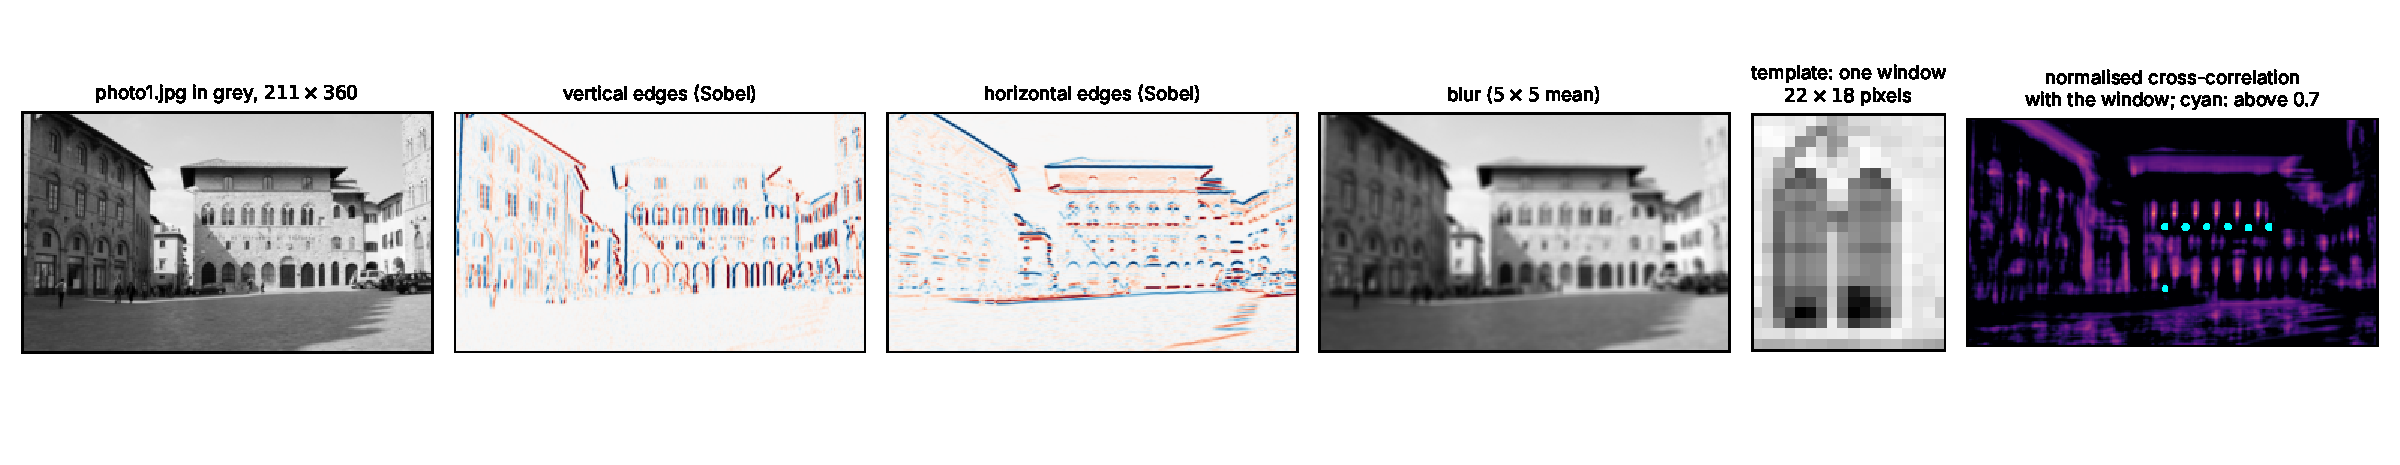
\includegraphics[width=0.99\textwidth]{week44_photo}
\end{center}
\small
The photograph from the week-45 folder (\texttt{photo1.jpg}, in grey,
$211\times360$ pixels).  The Sobel filters draw the vertical lines (walls,
window edges, people) and the horizontal ones (roof lines, floors,
arches); the blur removes the texture of the stone.  Right: one
double-arched window, $22\times18$ pixels, cut from the photograph and used
as the filter.  The normalised cross-correlation lights up at
\emph{every} window of that type -- six on the middle building, one on
the left -- and nowhere else above $0.7$.  A filter that finds windows is
the beginning of a filter that finds houses.
\end{frame}

\begin{frame}{From hand-made filters to learned ones}
\small
\begin{columns}[T]
\begin{column}{0.5\textwidth}
\begin{block}{What we did by hand}
Edge filters, a blur, a roof, a window: each is a small array of weights,
applied everywhere by the same formula.  Choosing them took us knowledge
of what a house looks like.
\end{block}
\begin{block}{What a CNN does}
It starts from \emph{random} filters and adjusts them by gradient descent
on the classification loss.  Trained on digits, the first-layer filters
become edge detectors -- opposed-sign pairs, oriented -- without anybody
asking for them (right, from the notebook).  The second layer combines
edges into corners and strokes, the third into shapes, and the dense
layers at the end decide between the classes.  A network trained on
houses would learn the window and the roof.
\end{block}
\end{column}
\begin{column}{0.48\textwidth}
\begin{center}
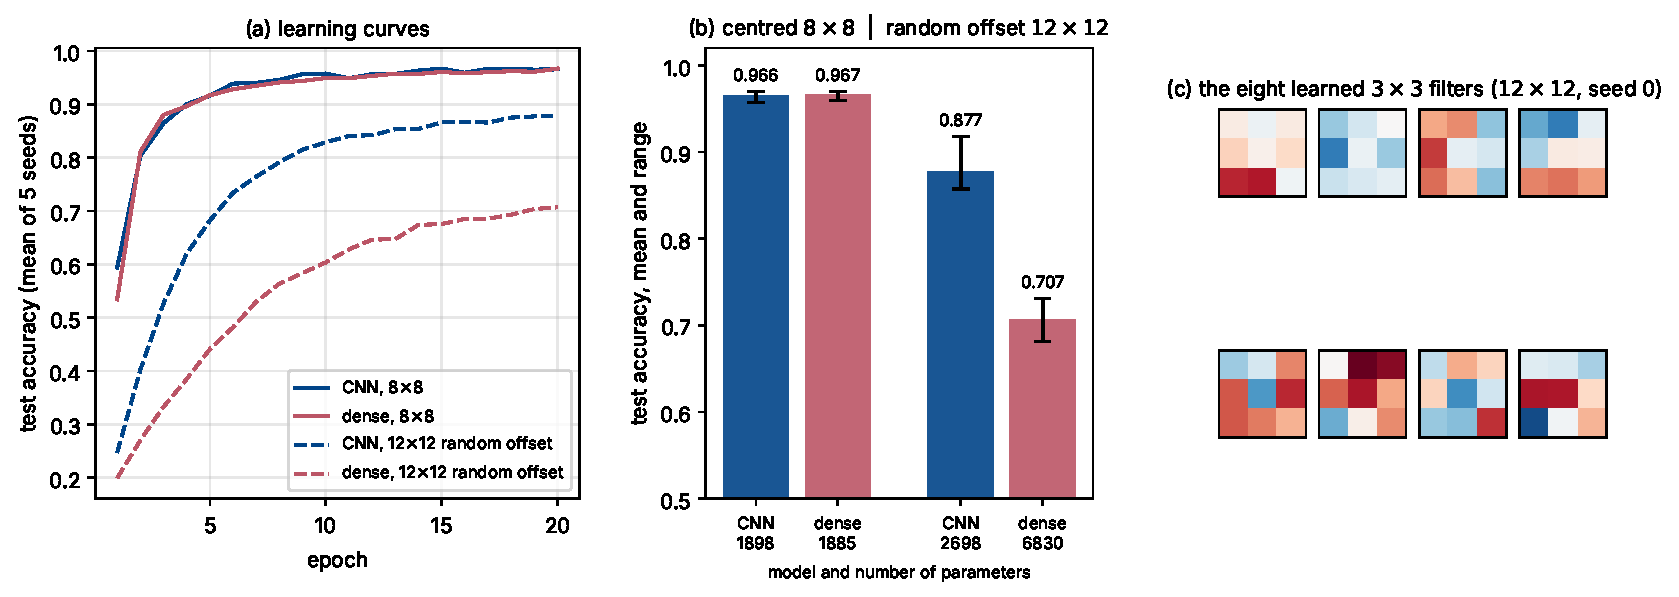
\includegraphics[width=0.98\textwidth]{week44_digits}\\
\scriptsize Our own NumPy network on the scikit-learn digits: learning
curves, centred against shifted digits, and the eight learned $3\times3$
filters of the first layer.
\end{center}
\end{column}
\end{columns}
\end{frame}

\begin{frame}{Why the same filter everywhere is the right choice: move the input, the map moves}
\begin{center}
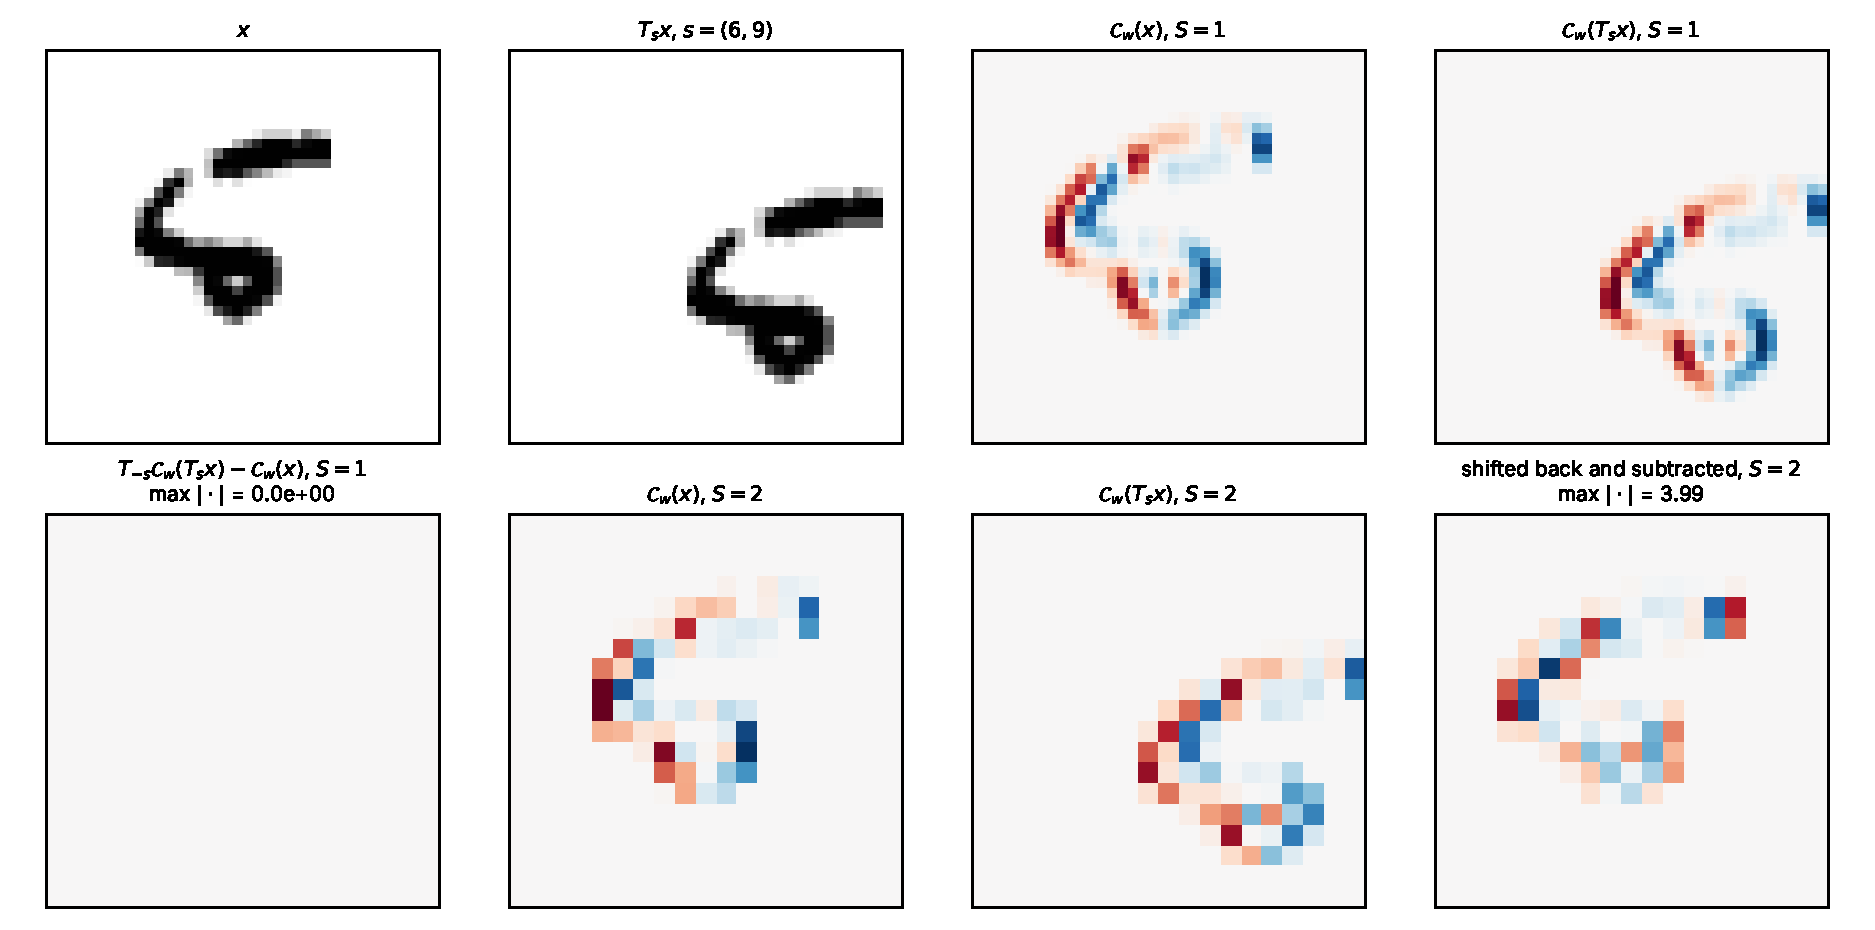
\includegraphics[width=0.60\textwidth]{week44_equivariance}
\end{center}
\small
The five is placed at two positions on a canvas; the vertical-edge map
slides with it and is otherwise \emph{identical} -- shifting the second
map back and subtracting gives exactly $0.0$ (top).  A filter that
responds to an edge responds to that edge wherever it is, because the same
weights are used at every position.  A dense layer has no such property:
it would have to learn the five at every position separately.  (The bottom
row shows that a stride of $2$ keeps the property only for even shifts --
one reason to stride with care.)
\end{frame}

\begin{insight}[reading a feature map]
\question{Why does the vertical-edge filter, whose rows read $(-1,0,1)$,
light up on the \emph{vertical} strokes of the five and of the house?
What does a ReLU after the layer do to such a map?  And what happens to
the roof filter if the house in the picture is twice as large?}
\answer{The filter is a difference between the pixel to the right and the
pixel to the left -- a derivative \emph{along a row}.  That derivative is
large where the intensity changes as we move sideways, which is at a
vertical stroke (the ink begins or ends), and zero on a horizontal stroke,
where every row is constant.  The sign says whether the ink begins (red)
or ends (blue); a ReLU keeps only one of the two, so a trained network
typically learns a filter \emph{and} its negative.  The roof filter is
$10\times16$ pixels and matches a roof of that size: a roof twice as large
gives a much weaker response.  Convolution handles \emph{position} for
free; size and rotation it does not -- a network learns those from
examples at several scales, or the data are augmented.}
\end{insight}

\begin{frame}{Pooling}
\small
\begin{columns}[T]
\begin{column}{0.5\textwidth}
Besides convolutions, \textbf{pooling} is the other building block.  A
pooling layer reduces the size of the feature maps by summarising small
regions: slide a window over the input and replace its content by one
number -- the \textbf{maximum} (max pooling, by far the most common) or
the \textbf{average}.
\begin{itemize}
  \item Works like a convolution, with the dot product replaced by a
        fixed function; \emph{no parameters} to train.
  \item Usually non-overlapping windows: $2\times2$ with stride $2$ halves
        width and height and keeps one of four numbers.
  \item Each channel is pooled separately: the depth does not change.
  \item Gives \emph{invariance to small translations}: if the largest value
        moves within its window, the output does not change.
\end{itemize}
\end{column}
\begin{column}{0.48\textwidth}
\begin{center}
\includegraphics[width=0.98\textwidth]{maxpooling}\\
\scriptsize Max and mean pooling with $3\times3$ windows and stride $3$
(Raschka et al.).
\end{center}
\end{column}
\end{columns}
\end{frame}

\begin{frame}{Pooling on our feature map (\texttt{week44\_pooling.pdf})}
\begin{center}
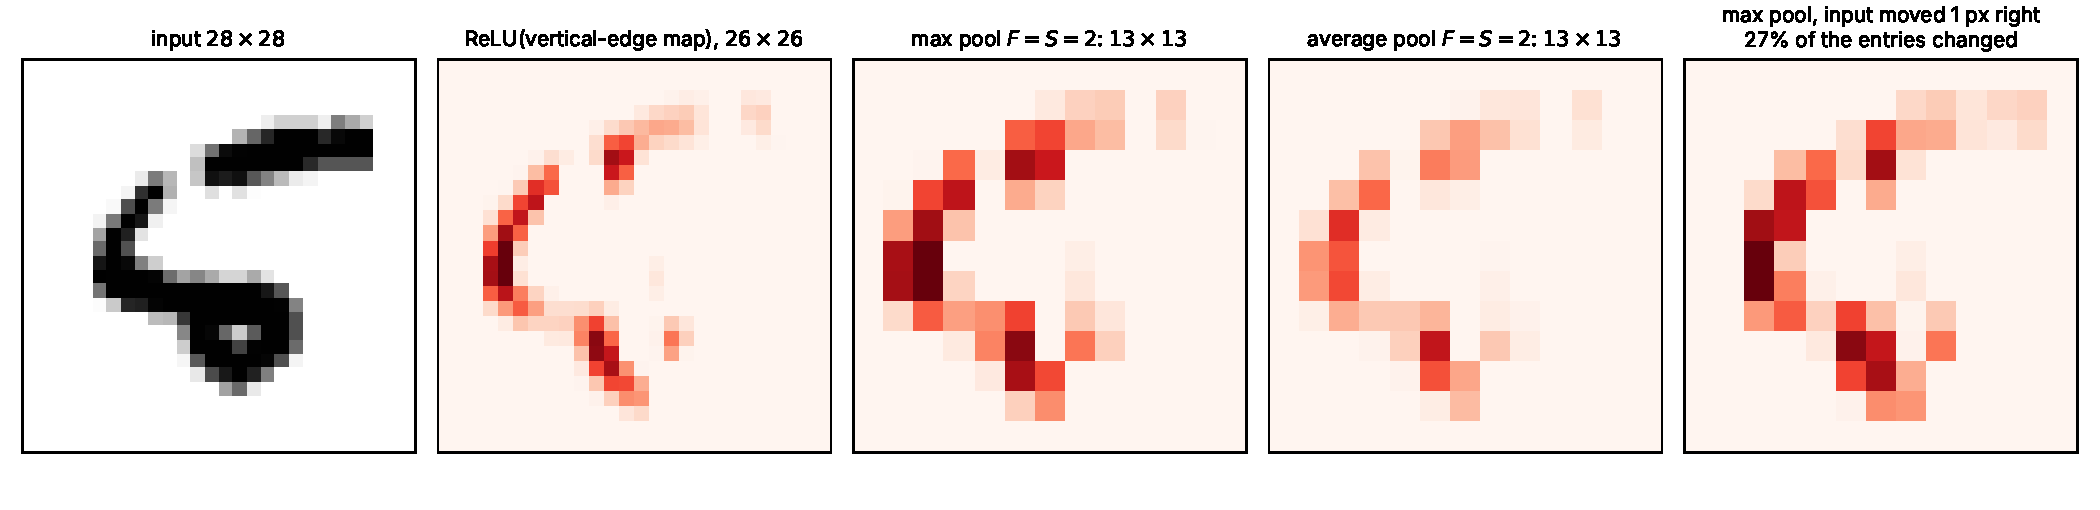
\includegraphics[width=0.98\textwidth]{week44_pooling}
\end{center}
\small
The vertical-edge map of the five after a ReLU ($26\times26$), max-pooled
and average-pooled with $2\times2$ windows and stride $2$ ($13\times13$),
and the max-pooled map when the digit is moved one pixel to the right:
$73\%$ of the pooled values are unchanged.  Max pooling keeps the strongest
response in each window; average pooling blurs.  After two conv--pool
blocks a $28\times28$ digit has become a stack of $7\times7$ maps, which is
flattened and handed to the dense layers.
\end{frame}

\begin{insight}[follow the sizes through the MNIST network]
\question{Input $28\times28\times1$.  Conv with $K=32$ filters, $F=3$,
$S=1$, $P=1$; max pool $2\times2$; conv with $K=64$, $F=3$, $S=1$, $P=1$;
max pool $2\times2$; flatten; dense to $1024$; dense to $10$.  Give the
size of every volume and the number of parameters of every layer.}
\answer{$28\times28\times1\to28\times28\times32$ ($320$ parameters)
$\to14\times14\times32$ (pool, $0$) $\to14\times14\times64$
($64\times(3\cdot3\cdot32+1)=18\,496$) $\to7\times7\times64$ (pool, $0$)
$\to3136$ (flatten) $\to1024$ ($3136\times1024+1024=3\,212\,288$)
$\to10$ ($10\,250$).  Total $3\,241\,354$, of which the two convolutional
layers hold $18\,816$, less than one per cent.  The dense layer after the
flattening holds almost everything -- keep this in mind when we look at
the results.}
\end{insight}

%% =====================================================================
\section{CNNs in code}
\begin{frame}{Building a CNN with TensorFlow/Keras or PyTorch: setting it up}
\small
\begin{itemize}
  \item The data are no longer a 2D feature matrix.  Each input is a stack
        of 2D arrays, one per colour channel, and the whole data set is a
        4D array (a \emph{tensor}):
        \[
          (n_{\mathrm{inputs}},\ n_{\mathrm{pixels,\,width}},\
          n_{\mathrm{pixels,\,height}},\ \mathrm{depth})
        \]
        in Keras; PyTorch puts the depth (channels) \emph{first},
        $(n_{\mathrm{inputs}},\mathrm{depth},\mathrm{height},\mathrm{width})$.
  \item MNIST: $28\times28$ grey images, depth $1$, so a tensor of shape
        $(60\,000,28,28,1)$ -- the same $784$ pixels per image as in
        Project 2, only not flattened.
  \item Images have strong \emph{local correlations}: a small part of the
        image varies little from its neighbours.  So instead of connecting
        every pixel to every neuron, each neuron sees a small region -- its
        \emph{receptive field} -- in all channels.
  \item Convolution (with a ReLU) and pooling are stacked in pairs.  By
        systematically reducing the size of the volume, the network builds
        representations of small parts of the image and assembles them
        into larger ones.  The last pooled volume is flattened and fed to
        ordinary dense layers with a softmax output.
\end{itemize}
\end{frame}

\begin{frame}{Training: nothing new}
\small
\begin{itemize}
  \item A convolutional layer is a linear map (the matrix $\bm{W}'$) followed
        by an activation; pooling is a fixed function.  The network is a
        composition of differentiable functions, so \textbf{backpropagation
        works unchanged}: the gradient with respect to the filter weights is
        itself a convolution (of the input with the error), and the gradient
        through a max pool goes to the element that won the maximum.
  \item The optimiser is the one of weeks 38--41: SGD or Adam on
        minibatches, with the softmax cross entropy of Chapter 5.
  \item The libraries do all of this by automatic differentiation
        (\texttt{loss.backward()} in PyTorch, \texttt{model.fit} in Keras).
\end{itemize}
\begin{block}{In the notebook, for those who want to see it}
\texttt{week44.ipynb} contains a complete NumPy implementation -- the
convolution as one matrix product (\texttt{im2col}), the backward pass,
max pooling and Adam -- with its gradients checked against finite
differences and the same network run on the digits and on MNIST.  It is
there to show that there is nothing in the library we could not write
ourselves; it is \emph{not} needed for Project 2.
\end{block}
\end{frame}

\begin{frame}[fragile]{A complete TensorFlow/Keras program for MNIST}
\lstset{basicstyle=\ttfamily\tiny}
\begin{columns}[T]
\begin{column}{0.56\textwidth}
\begin{lstlisting}
import numpy as np
from tensorflow import keras
from tensorflow.keras import layers
keras.utils.set_random_seed(1)

Xtr, ytr, Xte, yte = mnist_arrays()      # (N,1,28,28) in [0,1], from mnist.npz
std = lambda X: ((X - 0.1307) / 0.3081).astype("float32").transpose(0, 2, 3, 1)
Xtr, Xte = std(Xtr), std(Xte)            # (N, 28, 28, 1): channels LAST

model = keras.Sequential([
    keras.Input(shape=(28, 28, 1)),
    layers.Conv2D(32, 3, padding="same", activation="relu"),  # 28x28x32, 320 param.
    layers.MaxPooling2D((2, 2)),                              # 14x14x32
    layers.Conv2D(64, 3, padding="same", activation="relu"),  # 14x14x64, 18496
    layers.MaxPooling2D((2, 2)),                              # 7x7x64
    layers.Flatten(),                                         # 3136
    layers.Dense(1024, activation="relu"),                    # 3212288
    layers.Dropout(0.5),
    layers.Dense(10)])                                        # 10250, logits
model.compile(optimizer=keras.optimizers.Adam(1e-3),
              loss=keras.losses.SparseCategoricalCrossentropy(from_logits=True),
              metrics=["accuracy"])
model.summary()                                   # prints the parameter counts

for epoch in range(5):
    model.fit(Xtr, ytr, epochs=1, batch_size=64, verbose=0)
    print(epoch + 1, model.evaluate(Xte, yte, verbose=0)[1])
\end{lstlisting}
\end{column}
\begin{column}{0.42\textwidth}
\footnotesize
\begin{block}{Reading the program}
\begin{itemize}
  \item \texttt{Conv2D(K, F, padding="same")}: the cross-correlation of
        Part 2 with $K$ filters of size $F\times F$ and the padding that
        keeps the size; \texttt{MaxPooling2D((2, 2))}: the pooling.
  \item The comments give the volume after each layer and the parameter
        counts of Pause and think 4; \texttt{model.summary()} prints them.
  \item \texttt{from\_logits=True}: the network ends with scores and the
        loss applies the softmax itself.
  \item \texttt{Dropout(0.5)}: half of the $1024$ units switched off at
        random in each training step -- a regulariser for the layer that
        holds $99\%$ of the parameters; off at test time.
\end{itemize}
\end{block}
\end{column}
\end{columns}
\end{frame}

\begin{frame}[fragile]{The same network in PyTorch}
\lstset{basicstyle=\ttfamily\tiny}
\begin{columns}[T]
\begin{column}{0.56\textwidth}
\begin{lstlisting}
import torch, torch.nn as nn
torch.manual_seed(1)
Xtr, ytr, Xte, yte = mnist_arrays()               # (N,1,28,28): channels FIRST
std = lambda X: torch.tensor(((X - 0.1307) / 0.3081).astype("float32"))
Xtr, Xte, Ytr, Yte = std(Xtr), std(Xte), torch.tensor(ytr), torch.tensor(yte)

net = nn.Sequential(
    nn.Conv2d(1, 32, 3, padding=1), nn.ReLU(), nn.MaxPool2d(2, 2),   # (N,32,14,14)
    nn.Conv2d(32, 64, 3, padding=1), nn.ReLU(), nn.MaxPool2d(2, 2),  # (N,64,7,7)
    nn.Flatten(), nn.Linear(64 * 7 * 7, 1024), nn.ReLU(),
    nn.Dropout(0.5), nn.Linear(1024, 10))                            # logits
opt = torch.optim.Adam(net.parameters(), lr=1e-3)
lossf = nn.CrossEntropyLoss()                     # applies the softmax itself

for epoch in range(5):
    net.train()                                   # dropout on
    perm = torch.randperm(len(Xtr))
    for i in range(0, len(Xtr) - 64 + 1, 64):
        idx = perm[i:i + 64]
        opt.zero_grad(set_to_none=True)
        loss = lossf(net(Xtr[idx]), Ytr[idx])
        loss.backward()                           # backpropagation, by autograd
        opt.step()
    net.eval()                                    # dropout off
    with torch.no_grad():
        pred = torch.cat([net(Xte[i:i + 1000]).argmax(1) for i in range(0, 10000, 1000)])
    print(epoch + 1, (pred == Yte).double().mean().item())
\end{lstlisting}
\end{column}
\begin{column}{0.42\textwidth}
\footnotesize
\begin{block}{Reading the program}
\begin{itemize}
  \item \texttt{nn.Conv2d(C\_in, K, F, padding=P)}: input channels,
        filters, filter size, padding; layout $(N,C,H,W)$, channels
        first -- the one structural difference from Keras.
  \item PyTorch shows the loop that \texttt{model.fit} hides: a minibatch,
        the loss, \texttt{backward()}, a step of Adam.
  \item \texttt{nn.CrossEntropyLoss} expects logits; ending with a softmax
        applies it twice (a common, silent bug).
  \item \texttt{train()}/\texttt{eval()} switch dropout on and off; forget
        \texttt{eval()} and the test accuracy is measured with half the
        units missing.
  \item The dense baseline of Project 2 is one line:
        \texttt{nn.Sequential(nn.Flatten(), nn.Linear(784, 100), nn.ReLU(),
        nn.Linear(100, 10))}, same loop.
\end{itemize}
\end{block}
\end{column}
\end{columns}
\end{frame}

\begin{frame}{Results on MNIST (\texttt{week44\_mnist.pdf})}
\begin{center}
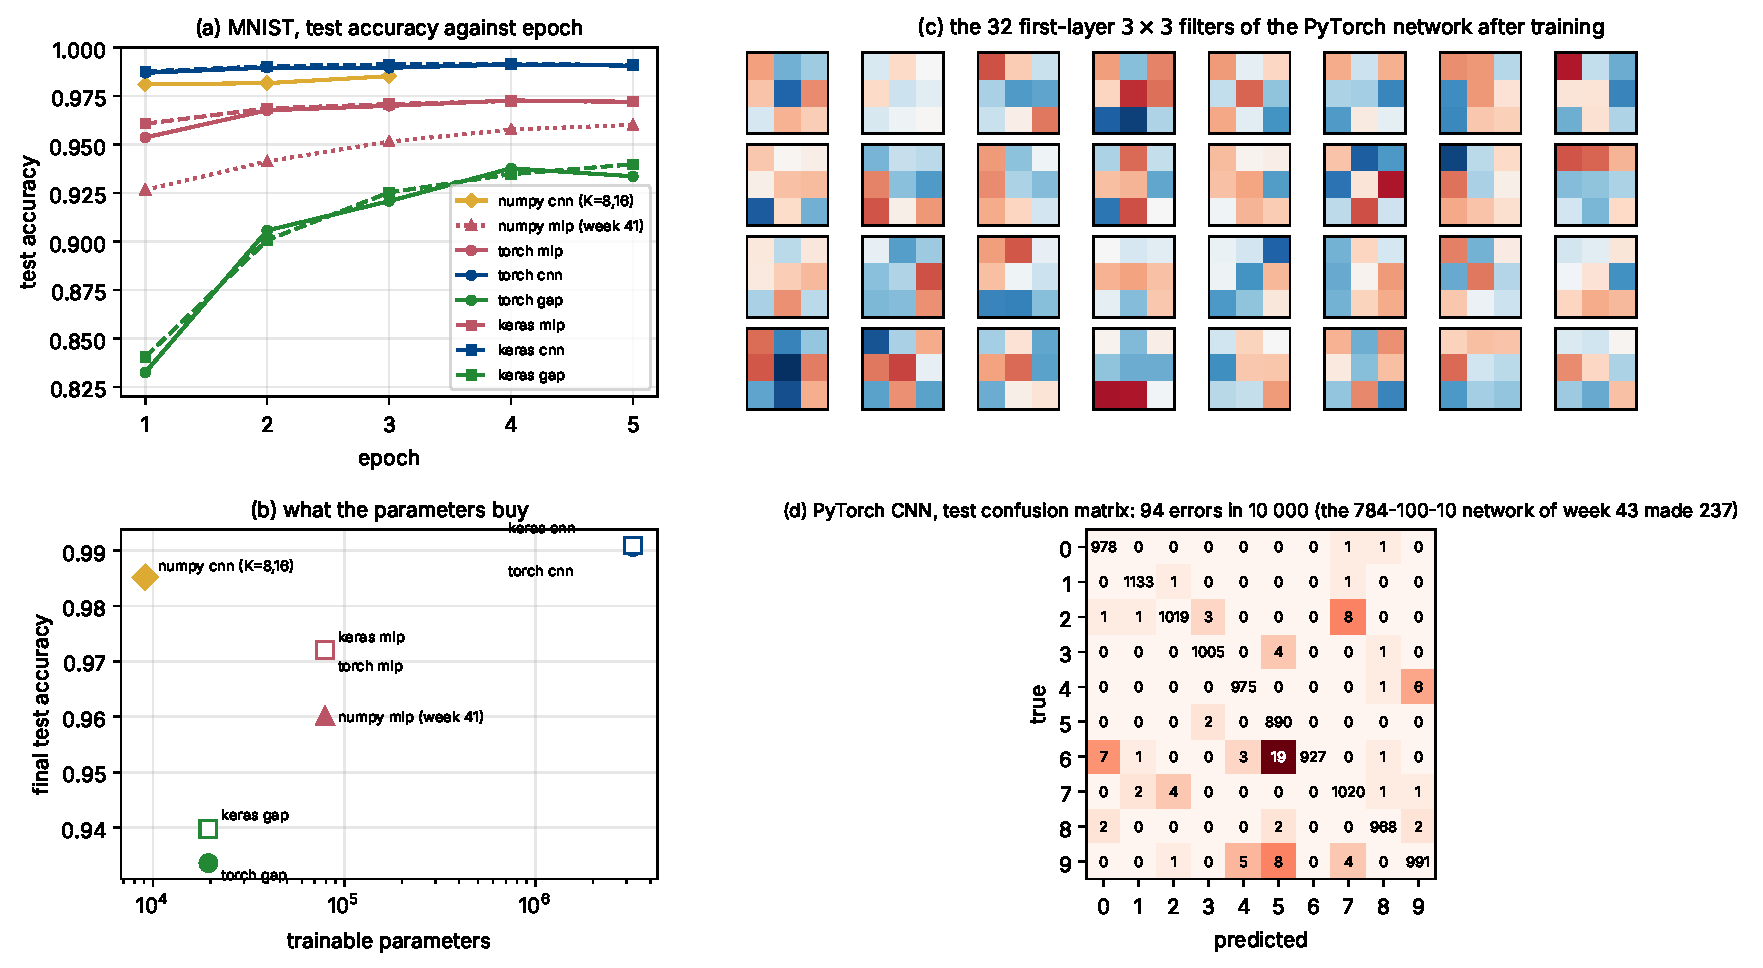
\includegraphics[width=0.90\textwidth]{week44_mnist}
\end{center}
\end{frame}

\begin{frame}{Reading the results}
\small
\begin{columns}[T]
\begin{column}{0.5\textwidth}
\begin{block}{Five epochs, Adam $10^{-3}$, batches of $64$, seed $1$; seconds per epoch on one CPU}
\setlength{\tabcolsep}{3pt}
\scriptsize
\begin{tabular}{@{}llrcc@{}}
\toprule
code & model & param. & test acc. & s/ep.\\
\midrule
NumPy & dense 784--100--10, SGD (week 41) & $79\,510$ & $0.9601$ & $1$\\
PyTorch & dense 784--100--10, Adam & $79\,510$ & $0.9720$ & $1$\\
Keras & dense 784--100--10, Adam & $79\,510$ & $0.9720$ & $3$\\
PyTorch & CNN of the listings & $3\,241\,354$ & $0.9906$ & $47$\\
Keras & CNN of the listings & $3\,241\,354$ & $0.9909$ & $37$\\
PyTorch & CNN, global average pooling & $19\,466$ & $0.9336$ & $19$\\
Keras & CNN, global average pooling & $19\,466$ & $0.9398$ & $18$\\
NumPy & CNN $K=8,16$ (3 epochs) & $9\,098$ & $0.9852$ & $71$\\
\bottomrule
\end{tabular}
\end{block}
\end{column}
\begin{column}{0.48\textwidth}
\footnotesize
\begin{itemize}
  \item \textbf{CNN against the Project 2 network:} same data, same
        optimiser, $94$ errors instead of $280$ on the $10\,000$ test
        images (week 43's dense network: $237$); the week-43 error bar
        $\sqrt{p(1-p)/n}\approx0.001$ says the gap is real.
  \item \textbf{PyTorch and Keras agree} to the noise of a stochastic
        optimiser ($0.9906$ against $0.9909$): different initialisations,
        shuffles and dropout masks, the same model.
  \item \textbf{Where the parameters are:} replace the $3.2$-million dense
        layer by the average of each $7\times7$ map (global average
        pooling, $19\,466$ parameters) and we lose five points in five
        epochs -- $99\%$ of the network does none of the convolutional
        work, but it is not pure waste either.
  \item \textbf{Our NumPy CNN} with $9\,098$ parameters beats the
        $79\,510$-parameter dense network: the \emph{architecture} is what
        the digits reward, not the count.  Forty times slower per epoch --
        the library is the tool.
\end{itemize}
\end{column}
\end{columns}
\end{frame}

\begin{frame}{Does it always help?  The experiment of Section 10.10}
\small
\begin{columns}[T]
\begin{column}{0.5\textwidth}
The scikit-learn digits ($8\times8$ pixels, $1797$ images): our NumPy CNN
against a dense network with the same number of parameters, five seeds.
\begin{center}
\scriptsize
\begin{tabular}{@{}llcc@{}}
\toprule
data & model & parameters & test accuracy\\
\midrule
centred $8\times8$ & CNN & $1898$ & $0.966$\\
centred $8\times8$ & dense & $1885$ & $0.967$\\
\midrule
random offset in $12\times12$ & CNN & $2698$ & $\mathbf{0.877}$\\
random offset in $12\times12$ & dense & $6830$ & $0.707$\\
\bottomrule
\end{tabular}
\end{center}
\end{column}
\begin{column}{0.48\textwidth}
\begin{itemize}
  \item On the digits as supplied -- small, centred, scaled -- the CNN is
        \emph{not} better.  There is no position to be invariant to, and a
        dense layer can afford one weight per pixel.
  \item Put the same digits at a random place in a slightly larger frame
        and the dense network loses $26$ points, the CNN $9$: the CNN
        learns each stroke once and finds it wherever it is; the dense
        network must learn every digit at every position.
  \item So: convolution is the right tool when the data have the structure
        it assumes -- patterns that can appear anywhere on a grid.  Images
        do; a table of unrelated measurements does not.
\end{itemize}
\end{column}
\end{columns}
\end{frame}

\begin{frame}[fragile]{Try at home: colour images, the CIFAR-10 data set (from the 2025 notes)}
\lstset{basicstyle=\ttfamily\tiny}
\begin{columns}[T]
\begin{column}{0.56\textwidth}
\begin{lstlisting}
import tensorflow as tf
from tensorflow.keras import datasets, layers, models

(train_images, train_labels), (test_images, test_labels) = datasets.cifar10.load_data()
train_images, test_images = train_images / 255.0, test_images / 255.0   # (50000,32,32,3)

model = models.Sequential()
model.add(layers.Conv2D(32, (3, 3), activation='relu', input_shape=(32, 32, 3)))
model.add(layers.MaxPooling2D((2, 2)))
model.add(layers.Conv2D(64, (3, 3), activation='relu'))
model.add(layers.MaxPooling2D((2, 2)))
model.add(layers.Conv2D(64, (3, 3), activation='relu'))
model.add(layers.Flatten())
model.add(layers.Dense(64, activation='relu'))
model.add(layers.Dense(10))
model.compile(optimizer='adam',
              loss=tf.keras.losses.SparseCategoricalCrossentropy(from_logits=True),
              metrics=['accuracy'])
history = model.fit(train_images, train_labels, epochs=10,
                    validation_data=(test_images, test_labels))
\end{lstlisting}
\end{column}
\begin{column}{0.42\textwidth}
\small
\begin{itemize}
  \item $60\,000$ colour images of $32\times32\times3$ in ten classes
        (airplane, automobile, bird, cat, \dots), $50\,000$ for training.
  \item The first \texttt{Conv2D} has $3\times3\times3+1=28$ parameters per
        filter, $896$ in all -- the answer of Pause and think 2.  With
        \texttt{padding} left at its default (``valid''), the sizes go
        $32\to30\to15\to13\to6\to4$.
  \item The program downloads the data ($170$ MB) and reaches about $70\%$
        test accuracy in ten epochs -- a much harder problem than MNIST,
        and where the dense network of Project 2 is hopeless.
\end{itemize}
\end{column}
\end{columns}
\end{frame}

%% =====================================================================
\section{Fourier filters}
\begin{frame}{Fourier filters: the convolution theorem}
\scriptsize
\begin{columns}[T]
\begin{column}{0.5\textwidth}
\begin{block}{The Fourier transform}
\[
  \hat f(\omega)=\int_{-\infty}^{\infty}f(t)\,e^{-i\omega t}\,dt,\qquad
  f(t)=\frac{1}{2\pi}\int_{-\infty}^{\infty}\hat f(\omega)\,e^{i\omega t}\,d\omega,
\]
and for $N$ samples the discrete transform (what \texttt{np.fft.fft}
computes),
\[
  X_k=\sum_{n=0}^{N-1}x_n\,e^{-2\pi ikn/N},\qquad
  x_n=\frac{1}{N}\sum_{k=0}^{N-1}X_k\,e^{2\pi ikn/N}.
\]
\end{block}
\begin{block}{The theorem}
For a convolution $(f*h)(t)=\int f(\tau)\,h(t-\tau)\,d\tau$, substitute
$s=t-\tau$ and the double integral factorises:
\[
  \boxed{\;\widehat{f*h}(\omega)=\hat f(\omega)\,\hat h(\omega)\;}
\]
Convolution in $t$ is \emph{multiplication} in $\omega$.  For sampled
data the same holds with the DFT and the \emph{circular} convolution
$(h\circledast x)_n=\sum_mh_m\,x_{(n-m)\bmod N}$.
\end{block}
\end{column}
\begin{column}{0.48\textwidth}
\begin{block}{Why this matters for filters}
A convolution filter $y=h*f$ therefore multiplies every frequency
component by one number,
\[
  \hat y(\omega)=H(\omega)\,\hat f(\omega),\qquad H=\hat h ,
\]
the \emph{frequency response}: $|H(\omega)|$ is the gain of the mode
$e^{i\omega t}$, $\arg H$ its phase shift.  Fourier modes are the
eigenfunctions of every convolution: $(h*e^{i\omega\,\cdot})(t)=H(\omega)\,e^{i\omega t}$.
\end{block}
\begin{block}{Two ways to filter, one operation}
\begin{itemize}
  \item in $t$: convolve with a kernel $h$ (what a CNN layer does);
  \item in $\omega$: transform, multiply by $H$, transform back.
\end{itemize}
The \emph{same} linear map: the second is how one designs or understands
a filter, the first is how a network applies it.
\end{block}
\end{column}
\end{columns}
\end{frame}

\begin{frame}{Example: a two-tone signal, a frequency mask, a three-point average (\texttt{week44\_fourier1d.pdf})}
\begin{center}
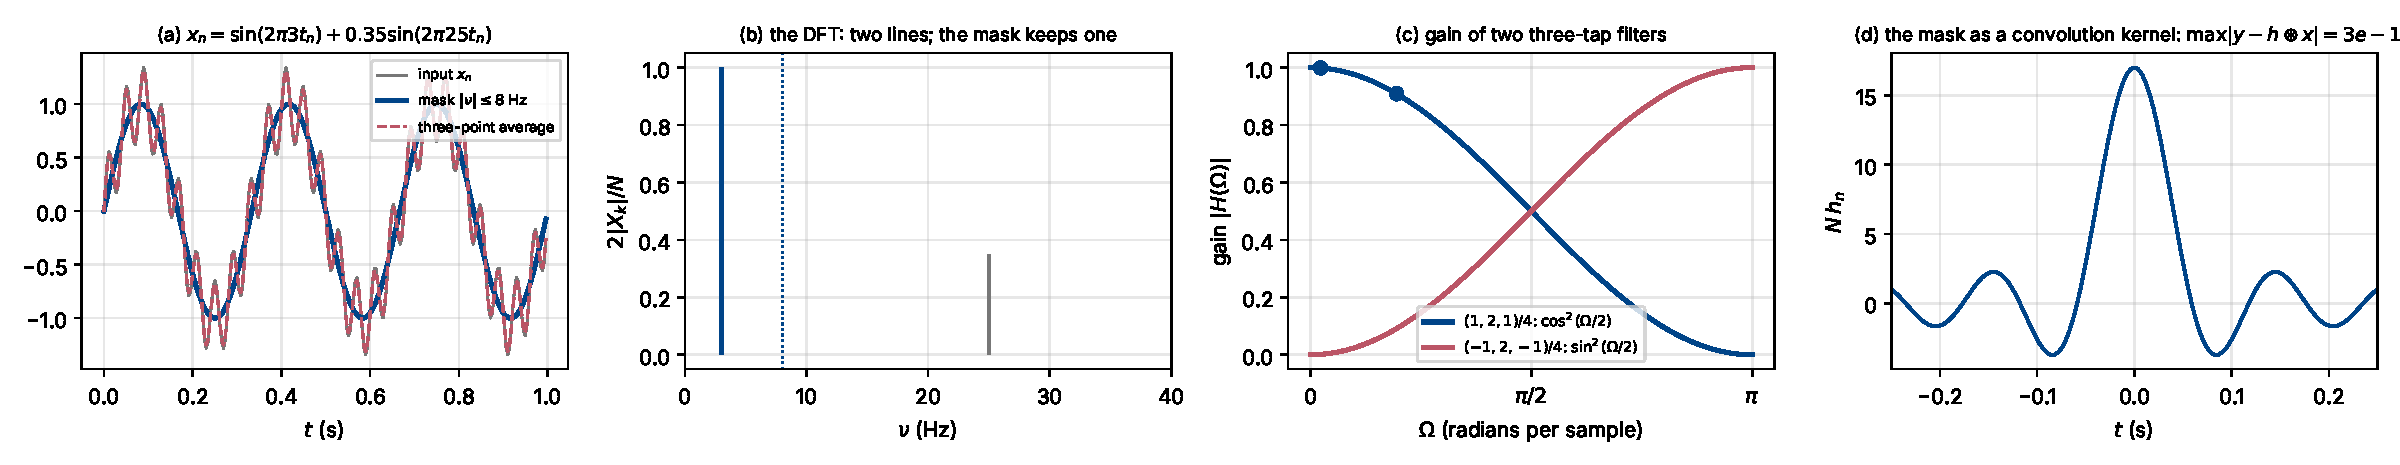
\includegraphics[width=0.99\textwidth]{week44_fourier1d}
\end{center}
\small
(a) $x_n=\sin(2\pi\,3t_n)+0.35\sin(2\pi\,25t_n)$, $N=256$ samples in one
second.  (b) Its DFT has two lines, at $3$ and $25$ Hz, with the two
amplitudes.  A \emph{mask} $H_k=1$ for $|\nu_k|\le8$ Hz, $0$ otherwise,
multiplied onto $X_k$ and transformed back, returns $\sin(2\pi\,3t_n)$ to
$2\times10^{-15}$: the $25$ Hz tone is gone.  (c) The three-point average
$y_n=\tfrac14x_{n-1}+\tfrac12x_n+\tfrac14x_{n+1}$ is a convolution with
$h=(1,2,1)/4$, whose response is $H(\Omega)=\cos^{2}(\Omega/2)$,
$\Omega=2\pi\nu/N$: gain $0.999$ at $3$ Hz, $0.909$ at $25$ Hz -- a gentle
low pass; $(-1,2,-1)/4$ has $\sin^{2}(\Omega/2)$, the complementary high
pass.  (d) The mask is \emph{also} a convolution: its kernel
$h=\mathrm{IDFT}(H)$ is a sampled $\sin(\omega_ct)/(\pi t)$ with long
oscillating tails, and $h\circledast x$ reproduces the masked result to
$3\times10^{-16}$.  Sharp in frequency means wide and oscillatory in time --
the origin of ``ringing'' near edges.
\end{frame}

\begin{frame}[fragile]{Linear against circular convolution, and the FFT as a fast convolution}
\scriptsize
\lstset{basicstyle=\ttfamily\tiny}
\begin{columns}[T]
\begin{column}{0.5\textwidth}
The DFT treats the record as periodic, so the product $H_kX_k$ is a
\emph{circular} convolution.  For $x=(1,2,3)$ and $h=(1,1)$ the linear
convolution is $x*h=(1,3,5,3)$, but
\begin{center}
\begin{tabular}{@{}lll@{}}
\toprule
FFT length & result & \\
\midrule
$N=3$ & $(4,3,5)$ & the last $3$ wrapped into the first bin\\
$N=4$ & $(1,3,5,3)$ & the full linear convolution\\
\bottomrule
\end{tabular}
\end{center}
Pad both sequences with zeros to $N\ge L_x+L_h-1$ and the FFT reproduces
the linear convolution exactly:
\begin{lstlisting}
x, h = np.array([1., 2., 3.]), np.array([1., 1.])
N = len(x) + len(h) - 1
y = np.fft.ifft(np.fft.fft(x, N) * np.fft.fft(h, N)).real   # [1. 3. 5. 3.]
\end{lstlisting}
\end{column}
\begin{column}{0.48\textwidth}
\begin{block}{Cost}
Direct convolution of $N$ samples with $K$ taps costs $O(NK)$; three FFTs
cost $O(N\log N)$.  For the $3\times3$ filters of a CNN the direct product
wins (and the libraries use it); for long kernels -- the sinc of the
previous frame, large blurs, audio filters -- the FFT wins by orders of
magnitude.
\end{block}
\begin{block}{Padding is the boundary model}
Circular: the DFT diagonalises the filter directly.  Zero padding (the $P$
of a CNN layer): pad to $N\ge L_x+L_h-1$, then crop.  Reflection: extend
the data first.
\end{block}
\begin{block}{Cross-correlation in Fourier language}
A CNN layer computes $z_n=\sum_rw_r\,x_{n+r}$, the convolution with the
\emph{reversed} kernel $h_r=w_{-r}$, so its response is
$A_k=\overline{W_k}$ for real weights: the same gain, the opposite phase
shift.  Symmetric kernels ($(1,2,1)$, the blur) do not notice.
\end{block}
\end{column}
\end{columns}
\end{frame}

\begin{frame}{The photograph in Fourier space (\texttt{week44\_fourier2d.pdf})}
\begin{center}
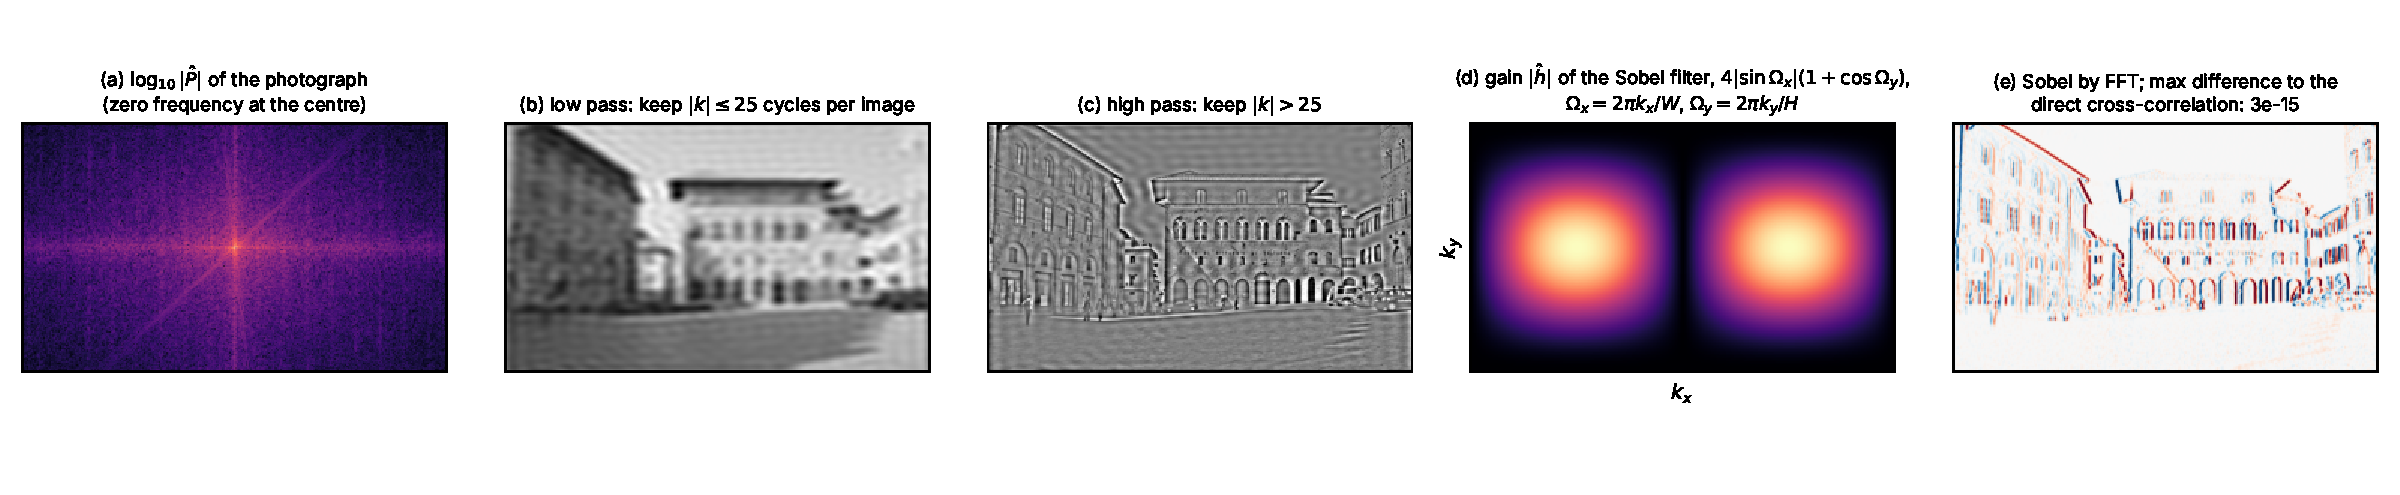
\includegraphics[width=0.99\textwidth]{week44_fourier2d}
\end{center}
\small
(a) $\log_{10}|\hat P(k_x,k_y)|$ of the $211\times360$ photograph: most of
the energy sits at low frequencies, with the bright horizontal and vertical
lines of the many vertical and horizontal edges.  (b) Keep only
$\sqrt{k_x^{2}+k_y^{2}}\le25$ cycles per image -- $2.6\%$ of the
coefficients -- and transform back: a blur, the low-pass filter of Part 3
done by multiplication.  (c) Keep the rest: the edges, a high-pass filter.
(d) The frequency response of the Sobel filter,
$|\hat h|=4|\sin\Omega_x|\,(1+\cos\Omega_y)$: zero on the axis
$\Omega_x=0$ (a horizontal edge is invisible to it), largest at
$|\Omega_x|=\pi/2$, and attenuated at high $\Omega_y$ by the $(1,2,1)$
smoothing.  (e) The Sobel map computed as
$\mathrm{IDFT}(\hat h\,\hat P)$ agrees with the direct cross-correlation to
$3\times10^{-15}$: the two routes are one operation.
\end{frame}

\begin{frame}{A CNN layer in Fourier language}
\scriptsize
\begin{columns}[T]
\begin{column}{0.5\textwidth}
\begin{block}{The linear stage is channel mixing, frequency by frequency}
With circular boundaries and stride $1$, the layer
$z_a[n]=b_a+\sum_b\sum_rw_{ab}[r]\,x_b[n+r]$ becomes, after a DFT,
\[
  \bm{Z}[k]=\bm{A}[k]\,\bm{X}[k],\qquad
  \bm{A}[k]\in\mathbb{C}^{C_{\mathrm{out}}\times C_{\mathrm{in}}},
\]
one small matrix per frequency, with entries
$A_{ab}[k]=\sum_rw_{ab}[r]\,e^{2\pi ikr/N}$.  Different frequencies never
mix in the linear stage.
\end{block}
\begin{block}{What a short kernel can and cannot do}
A $3\times3$ kernel has a response that is a trigonometric polynomial of
degree one in each direction -- the smooth surfaces of panel (d).  Its
frequency bins cannot be set independently: a sharp cutoff like the mask
of the $1$D example needs a long kernel, or a frequency-space layer.
\end{block}
\end{column}
\begin{column}{0.48\textwidth}
\begin{block}{Where the frequency picture stops}
\begin{itemize}
  \item \textbf{The ReLU creates new frequencies}:
        $\max(0,\sin t)=\tfrac12\sin t+\tfrac12|\sin t|$ has a constant
        term and all even harmonics.  A full CNN has no single response
        $H$; the linear stage of each layer does.
  \item \textbf{Stride and pooling change the sampling grid}: keeping
        every second sample folds frequencies above the new Nyquist limit
        back down -- $\cos(0.2\pi n)$ and $\cos(0.8\pi n)$ become
        identical.  A low pass before downsampling (a blur before the
        pool) removes the aliases; a learned strided filter does not do
        this by itself.
\end{itemize}
\end{block}
\begin{block}{Training in Fourier words}
Gradient descent on $w[r]$ moves the response
$A(\Omega)=\sum_rw[r]e^{i\Omega r}$ at all frequencies at once.  What it
converges to depends on the task: the edge detectors of Part 3 are
directional high-pass filters, learned because edges separate digits.
\end{block}
\end{column}
\end{columns}
\end{frame}

\begin{frame}{How Fourier filters are used, 1: signal processing and differential equations}
\small
\begin{itemize}
  \item \textbf{Denoising and band selection.}  A mask or a smooth response
        $H$ removes what lies outside the band of interest: the $25$ Hz
        tone of the example, the stone texture of the photograph, the
        mains hum in a measurement.  The choice of $H$ is the model of
        what is signal and what is noise; the transform itself decides
        nothing.
  \item \textbf{Fast convolution.}  A long kernel -- a wide blur, a sinc, an
        audio reverberation -- is applied with three FFTs in $O(N\log N)$
        instead of $O(NK)$.
  \item \textbf{Solving differential equations.}  The Poisson problem of
        week 43, $-u''=f$ on $(0,1)$ with $u(0)=u(1)=0$: expand in the
        sine modes that satisfy the boundary conditions,
        $f=\sum_nf_n\sin(n\pi x)$, and since
        $-\frac{d^{2}}{dx^{2}}\sin(n\pi x)=(n\pi)^{2}\sin(n\pi x)$,
        \[
          u(x)=\sum_{n=1}^{\infty}\frac{f_n}{(n\pi)^{2}}\sin(n\pi x):
        \]
        the inverse operator is a \emph{filter} that damps mode $n$ by
        $1/(n\pi)^{2}$.  (Fixed boundaries break translation invariance,
        so this is a sine series, not a convolution on the whole line.)
  \item \textbf{Reading a filter.}  The response $H$ of a kernel says what
        it does -- low pass, high pass, oriented -- more directly than its
        weights: $(1,2,1)/4$ is $\cos^{2}(\Omega/2)$, Sobel is
        $4|\sin\Omega_x|(1+\cos\Omega_y)$.
\end{itemize}
\end{frame}

\begin{frame}{How Fourier filters are used, 2: inside convolutional networks}
\small
\begin{itemize}
  \item \textbf{Anti-aliasing.}  A blur before every stride-2 pool, so that
        a shifted input gives a shifted output instead of an aliased one
        (Zhang, ICML 2019).
  \item \textbf{Spectral pooling.}  Reduce the resolution by truncating the
        DFT of a feature map instead of taking maxima: the low frequencies
        are kept exactly (Rippel, Snoek and Adams, NeurIPS 2015).
  \item \textbf{Learning the filters in frequency space.}
        $z=\mathrm{IDFT}\bigl[R_\theta[k]\,X[k]\bigr]$ with one learned
        matrix per retained frequency -- a \emph{global} kernel with few
        parameters.  This is the layer of the Fourier neural operator,
        which learns the solution operator of a PDE from examples (Li et
        al.\ 2021).
  \item \textbf{Fourier-weighted losses} for reconstruction tasks.  By
        Parseval, $\frac1N\sum_n|e_n|^{2}=\frac{1}{N^{2}}\sum_k|E_k|^{2}$
        for the error $e=y-t$; weights $q_k$ on the spectrum decide which
        frequencies the training must get right.
\end{itemize}
\begin{block}{What to remember}
A Fourier transform is a change of representation and loses nothing; a
filter is a choice of what to keep.  Convolution with $h$ and
multiplication by $H=\hat h$ are the same operation.  A CNN learns $H$
one short kernel at a time, with non-linearities and pooling in between
that the frequency picture does not cover.  The derivations are in
Section 10.13 of the lecture notes.
\end{block}
\end{frame}

\begin{insight}[two sequences through two filters]
\question{Send the alternating sequence $x_n=(-1)^{n}$ and the constant
sequence $x_n=1$ through the three-point average $(1,2,1)/4$ and through
$(-1,2,-1)/4$.  What comes out, and why does the Sobel response vanish
on the line $\Omega_x=0$?}
\answer{The alternating sequence is the mode $\Omega=\pi$: the average
has $\cos^{2}(\pi/2)=0$, so it is removed entirely
($\tfrac14-\tfrac12+\tfrac14=0$ at every $n$); $(-1,2,-1)/4$ has
$\sin^{2}(\pi/2)=1$ and passes it unchanged.  The constant sequence is
$\Omega=0$: the average passes it ($\cos^{2}0=1$) and the high pass kills
it ($-\tfrac14+\tfrac12-\tfrac14=0$).  The two gains add to one -- the
filters split the signal into its smooth and its varying part.  The Sobel
filter's columns are $(-1,0,1)$: a central difference along the row, whose
response is $2i\sin\Omega_x$ -- zero at $\Omega_x=0$, which is every
pattern that does not change along a row.  A horizontal edge is such a
pattern, so it is invisible to $W_{\mathrm{vert}}$ and needs
$W_{\mathrm{hor}}$ -- exactly what the house showed.}
\end{insight}

%% =====================================================================
\begin{frame}{Where this is going: tomorrow, the exercises, Project 2}
\small
\begin{columns}[T]
\begin{column}{0.5\textwidth}
\begin{block}{Tomorrow: cross-validation for your Project 2 network}
Twenty minutes of theory -- what the $k$-fold estimate is, its error bar,
the one-standard-error rule, why the scaler goes inside the fold -- then
the six questions of exercise 1 and your own network inside
\texttt{scikit-learn}'s \texttt{KFold}, \texttt{cross\_validate},
\texttt{GridSearchCV} and \texttt{validation\_curve} (exercise 2).
\end{block}
\begin{block}{Exercises week 44 (deadline Friday October 30)}
1: six questions on cross-validation.  2: your Project 2 regression
network cross-validated by \texttt{scikit-learn}.  3 (optional): the
MNIST classifier.  4 (optional): the loop written by hand.  Declare your
use of LLMs.
\end{block}
\end{column}
\begin{column}{0.48\textwidth}
\begin{block}{Project 2 (deadline November 6)}
Asks for a dense network and logistic regression, not a CNN.  A group that
wants to add today's CNN as a comparison is welcome to -- cross-validated
the same way, and compared honestly.
\end{block}
\begin{block}{Next Monday, week 45}
Chapter 11, recurrent neural networks -- sequences, the unrolled graph,
backpropagation through time -- and time for Project 2 questions.
\end{block}
\begin{block}{Reading}
Chapter 10, Sections 10.1--10.7 and 10.10--10.13 (10.13: Fourier
filters); Goodfellow et al.\ Chapter 9; Raschka et al.\ Chapters 14--15.
For tomorrow: Sections 2.12, 3.14 and 8.12.
\end{block}
\end{column}
\end{columns}
\end{frame}

\begin{frame}{Summary of week 44}
\small
\begin{itemize}
  \item A CNN is a neural network that \emph{assumes its input is an
        image}: neurons see a small neighbourhood (locality) and the same
        weights are used everywhere (parameter sharing).  The parameter
        count no longer depends on the image size.
  \item Convolution: $y(i)=\sum_kw(k)\,x(i-k)$ -- polynomial multiplication
        is the first example, a Toeplitz matrix the second way to write it.
        Padding supplies the missing indices, the stride decides how far
        the filter moves, and the libraries compute the cross-correlation
        $\sum_kw(k)\,x(i+k)$ under the name convolution.
  \item In two dimensions: slide an $F\times F$ filter over the image,
        dot product at every position; output size
        $(W_1-F+2P)/S+1$, depth $K$, parameters $(F\times F\times D_1)K+K$.
  \item Filters detect things: edges on a digit and a house, a roof, a
        window in a photograph.  A CNN \emph{learns} its filters, and learns
        edge detectors first.  Pooling discards position in small steps.
  \item PyTorch and Keras: a few lines for the network, the familiar loop
        for training; $99\%$ on MNIST against $97\%$ for the Project 2
        network, with the same optimiser.  Every number has hyperparameters
        behind it that nobody chose -- tomorrow is about choosing them.
  \item Fourier: convolution with $h$ is multiplication by $H=\hat h$; a
        filter is a choice of which frequencies to keep; a short CNN kernel
        is a smooth response, learned one weight at a time, with
        non-linearities and pooling in between that Fourier does not see.
\end{itemize}
\end{frame}

\end{document}
